\section{wissenschaftliches Arbeiten}
\subsection{Einf\"uhrung}
\begin{frame}{wissenschaftliches Arbeiten mit \LaTeX}
 Wie bereits angek\"undigt, \LaTeX~ist der Standard f\"ur wissenschafliche Arbeiten in den MINT F\"achern und das nicht ohne Grund. \LaTeX~bietet zahlreiche Tools um wissenschaftliches Arbeiten zu unterst\"utzen.\\\vspace{3mm} In der Regel beginnen wissenschaftliche Arbeiten mit einem Deckblatt.
\end{frame}
\subsection{Deckblatt}
\begin{frame}{Deckblatt}
    \LaTeX~bietet zahlreiche Optionen um Informationen f\"ur das Deckblatt einzutragen.
    \begin{itemize}
        \item \cblue\textbackslash author\black\{Name\}~- Name des Autors (mehrere Autoren k\"onnen mit \cblue\textbackslash and\black~verkn\"upft werden)
        \item \cblue\textbackslash date\black\{Datum\}~- Datum des Dokuments (kann mit \cblue\textbackslash today\black~verkn\"upft werden um das aktuelle Datum einzutragen)
        \item \cblue\textbackslash title\black\{Titel\}~- Titel des Dokuments
        \item \cblue\textbackslash subtitle\black\{Untertitel\}~- Untertitel des Dokuments (nur in Dokumentklasse scrartcl)
    \end{itemize}
    All diese Befehle m\"ussen \textbf{VOR} der \cpurple document\black-Umgebung stehen. Mit dem Befehl \cblue\textbackslash maketitle\black~\textbf{IN} der \cpurple document\black-Umgebung generiert man den Titel.
\end{frame}
\begin{frame}{Deckblatt - Beispiel}
    \begin{columns}
    \begin{column}{.4\textwidth}
        \% Usepackages \\
        \cblue\textbackslash author\black\{Hans M\"uller\}\\
        \cblue\textbackslash date\black\{28.10.2016\}\\
        \cblue\textbackslash title\black\{Ein toller Titel\}\\
        \cblue\textbackslash subtitle\black\{Der Untertitel\}\\
        \cblue\textbackslash begin\black\{\cpurple document\black\}\\
        \cblue\textbackslash maketitle\black\\
        \cblue\textbackslash end\black\{\cpurple document\black\} 
    \end{column}
    \begin{column}{.6\textwidth}
    \begin{figure}
        \centering
        
\includegraphics[width=6cm]{images/title.jpg}
        \caption{Der Output des Codes}
    \end{figure}
    \end{column}
    \end{columns}
\end{frame}
\subsection{ToC, Section, Subsection}
\begin{frame}{ToC, Section, Subsection}
    Wir kennen bereits aus \hyperlink{sec:toc}{einem vorherigen Kapitel} den Table of Contents mit den Sections und Subsections. Auf diesem Wissen bauen wir nun auf. \\\vspace{3mm}\textit{Zur Erinnerung:}\\Mit dem Befehl \cblue \textbackslash section\black~definiert man eine \"Uberschrift, mit \cblue \textbackslash subsection\black~eine Unter\"uberschrift, mit \cblue \textbackslash subsubsection\black~eine Unterunter\"uberschrift usw.\\\vspace{3mm}
    Mit \cblue \textbackslash tableofcontents\black~l\"asst sich ein Inhaltsverzeichnis erstellen.
\end{frame}
\begin{frame}{ToC, Section, Subsection - Beispiel}
    \begin{columns}
    \begin{column}{.4\textwidth}
    \footnotesize\cblue \textbackslash section\black \{Eine tolle \"Uberschrift\}\\
    \cblue \textbackslash subsection\black\{Eine Unter\"uberschrift\}\\
    \cblue\textbackslash subsubsection\black\{Eine \"Uberschrift dritter Ordnung\}\\
    \cblue\textbackslash subsection\black\{Verschachtelung ist toll!\}\\
    \cblue\textbackslash section*\black\{Keine Nummerierung \cred\$\cblue\textbackslash rightarrow\cred\$\black~auch nicht im ToC\}
    \cblue\textbackslash section\black\{\"Uberschrift erster Ordnung\}
    \end{column}
    \begin{column}{.6\textwidth}
    \begin{figure}
        \centering
        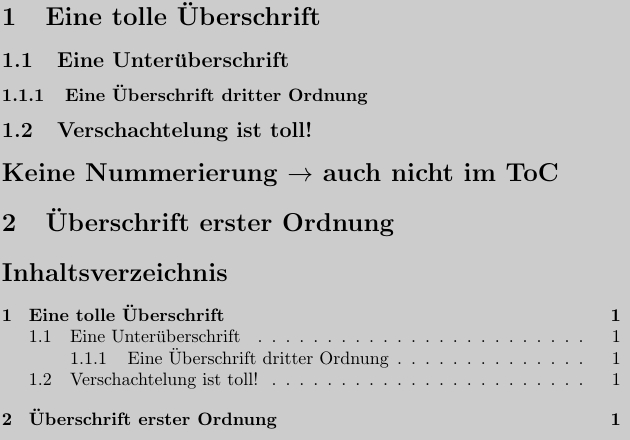
\includegraphics[width=6cm]{images/toc.jpg}
        \caption{Zugeh\"origer Table of Contents}
    \end{figure}
    \end{column}
    \end{columns}
    Falls keine Nummerierung in der \"Uberschrift gew\"unscht ist, ist dies mit einem * nach dem Befehl zu realisieren.
\end{frame}
\subsection{Referenzen und Verlinkungen}
\begin{frame}{Referenzen und Verlinkungen}
    Wissenschaftliche Arbeiten enthalten oft Darstellungen, Formeln etc. auf welche sich der Autor im Text bezieht. F\"ur eine bessere Leseerfahrung bietet \LaTeX~die M\"oglichkeit Referenzen zu setzen, welche bei einem Mausklick zu dem referenzierten Objekt springen.\\\vspace{4mm}
    Mit \cblue\textbackslash label\black\{Bezeichner\} setzen wir einen Punkt f\"ur eine Referenz. Mit \cblue\textbackslash ref\black\{Bezeichner\} wird auf den Punkt referenziert.\\
    Die Bezeichner sind \textit{intern} und tauchen i.d.R. in der kompellierten Datei nicht auf.\\\vspace{4mm}
    Generell bietet sich an, die Bezeichner m\"oglichst eindeutig zu benennen. Das Format \textit{Dateik\"urzel:Name} hat sich hierbei eingeb\"urgert, Bsp: \cblue\textbackslash label\black\{\textit{img:birds}\} f\"ur ein Bild von V\"ogeln.
\end{frame}
\todo{Bibtex}
\todo{Referenzen}